\documentclass[border=4pt]{standalone}
\usepackage{pgfplots}
\pgfplotsset{compat=1.18}

\begin{document}
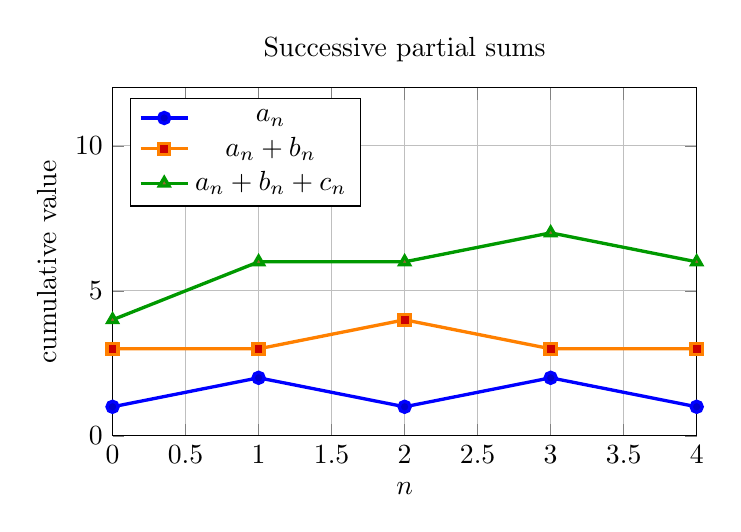
\begin{tikzpicture}
  \begin{axis}[
    stack plots=y,
    width=9cm,
    height=6cm,
    xmin=0,
    xmax=4,
    ymin=0,
    ymax=12,
    xlabel={$n$},
    ylabel={cumulative value},
    title={Successive partial sums},
    grid=major,
    legend pos=north west
  ]
    \addplot+[blue,very thick,mark=*] coordinates {(0,1) (1,2) (2,1) (3,2) (4,1)};
    \addplot+[orange,very thick,mark=square*] coordinates {(0,2) (1,1) (2,3) (3,1) (4,2)};
    \addplot+[green!60!black,very thick,mark=triangle*] coordinates {(0,1) (1,3) (2,2) (3,4) (4,3)};
    \legend{$a_n$,$a_n+b_n$,$a_n+b_n+c_n$}
  \end{axis}
\end{tikzpicture}
\end{document}
